\chapter{Observations}
 %This section  .... table \ref{table:2} \cite{r2}
\section{Insights from Computational Analysis} 

From the computation results, it is clear that Logistic Regression performs better than other models, and gains the top CV accuracy of 90.11\%. This indicates that Logistic Regression gives the highest generalization performance over all of the models. SVM is a close second with CV accuracy of 88.52\%, showing that it is good at learning digest intricate information in the data. Gradient Boost, Random Forest, XGBoost and Naive Bayes  classifiers also yield comparable performance (87\%-80.0\% CV accuracies). These models work well, though they don’t take the top two spots. Here by comparing the CV accuracies, we notice that SVM does fairly close at 88.52\% and KNN and Decision Tree have significantly lower CV accuracies of 80.5\% and 72.57\% respectively meaning that they do worse in generalizing on unseen data than the other methods.




\section{Limitations} 

Models have different capabilities but there are a number of limitations. First, the analysis was made using cross-validation accuracy and not the whole model performance. Class imbalance, overfitting or data-specif characteristics in the domain can have an impact on their performance when employed in deployment. Also, the method does not consider hyperparameter tuning for each model. These can potentially improve the performance of the methods. Finally, the model complexity and explainability of some models such as Gradient Boosting and XGBoost can make them less useful in practice for certain problem settings than simpler models like Logistic Regression or Naive Bayes.


\section{Results}



The results of our experiments (cross-validation accuracies) suggest that Logistic Regression and SVM are the two top models for this task. These are both reasonably simple yet powerful models, that were shown to achieve high accuracy with low computational cost. We find that Naive Bayes, Gradient Boosting and Random Forest give good results but not better than Logistic Regression and SVM in our context. The KNN and Decision Tree methods are outperformed by the latter, and it may indicate that more complex techniques suit to the specific nature of this problem better, probably because they capture intricate patterns/interplays present in the data.

\begin{table}[ht]
\centering
\begin{tabular}{|l|c|}
\hline
\textbf{Model}            & \textbf{CV Accuracy} \\ \hline
Logistic Regression        & 0.90              \\ \hline
SVM         & 0.86              \\ \hline
Gradient Boosting                & 0.88              \\ \hline
Random Forest                         & 0.88              \\ \hline
XGBoost             & 0.88              \\ \hline
Naive Bayes                    & 0.87              \\ \hline
KNN                         & 0.80              \\ \hline
Decision Tree              & 0.73              \\ \hline
\end{tabular}
\caption{Cross-Validation Accuracy of Various Models}
\label{tab:cv_accuracy}
\end{table}

 
\begin{figure}
    \centering
    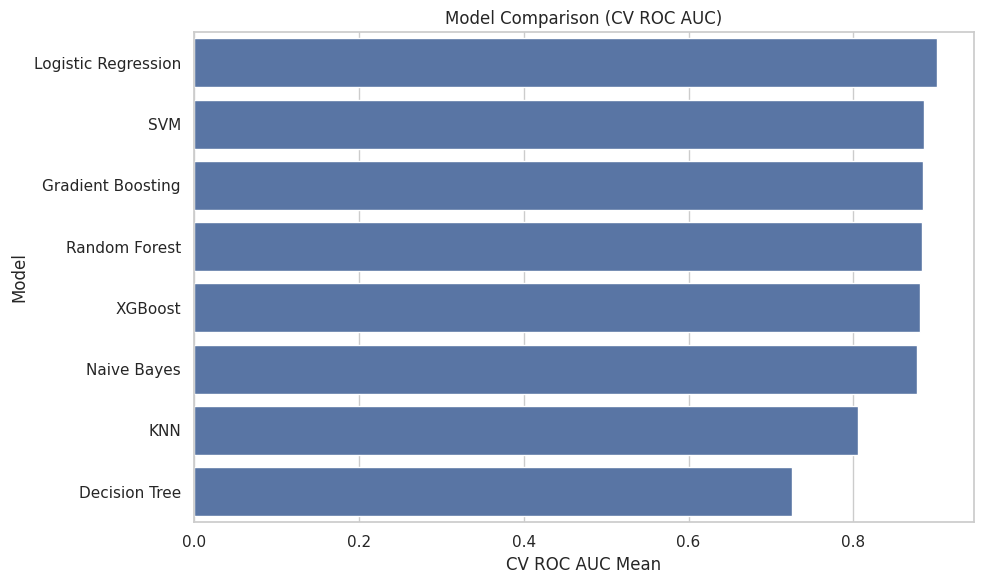
\includegraphics[width=0.75\linewidth]{Chap4/model-comparision.png}
    \caption{Compare model}
    \label{fig:placeholder}
\end{figure}

\section{Web Application}
\begin{figure}
    \centering
    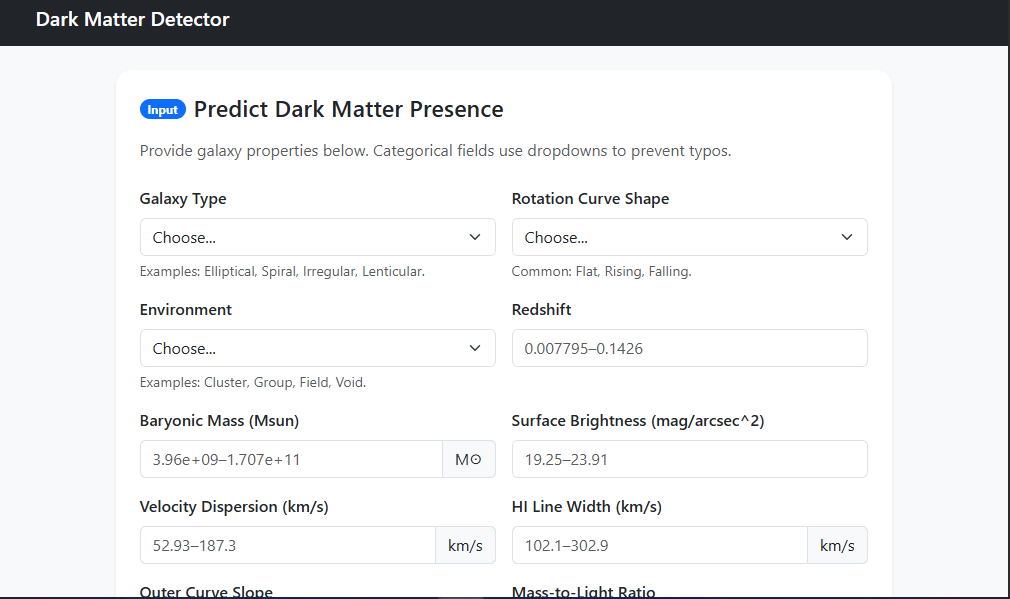
\includegraphics[width=0.5\linewidth]{Chap4/web-application.png}
    \caption{Web application of dark matter detector}
    \label{fig:placeholder}
\end{figure}
The Dark Matter Detector site is a web based, freely available tool that uses a very user-friendly and intuitive user interface to calculate the probability dark matter is detected given arbitrary date for R V, Reff, $\Sigma$g ±. The features to be chosen by the user for classification are basic properties of a galaxy such as its type (e.g., Elliptical, Spiral, Irregular or Lenticular) and nature of environment it reside in –cluster, group, field or void. And, users can provide their baryonic mass in solar masses, the velocity dispersion in km/s and the outer curve slope, which is a good representation of how the rotation curve of your galaxy behaves at its outskirts.

Other important parameters are the rotation curve type (flat, rising, falling, etc.) and whether or not we need to plot a gap (it can highlight with clip marks if you select yes). The redshift is another important parameter that shows the distance and motion of galaxy with respect to Earth. The surface brightness S in units of magnitudes per square arc-second and the HI line width provide an estimate of the galaxy luminosity and also on velocity distribution of hydrogen gas inside a galaxy. Finally, the user must specify the mass-to-light ratio, an important parameter in determining how much dark matter there is on the basis of its visible mass and the gravitational impact of the galaxy.

By imputing these galaxy properties, the website hopes to make a prediction for the probability of dark matter presence and contribute to human understanding of how a galaxy’s visible properties relate to the invisible substance that determines its evolution. This is an essential tool to push forward the field of dark matter astrophysics.

 